\section*{Análise de Algoritmos}

\begin{frame}
\begin{block}{Como construir algoritmos?}
	\begin{itemize}
		\item Podemos implementar o primeiro pensamento que vier em nossas mentes...
		
		\item Como saber se esse pensamento foi ‘bom’ como comparar dois algoritmos que resolvem o mesmo problema e determinar que o primeiro é melhor que o segundo de forma sistemática?
		
		\item Sugestões?
	\end{itemize}
\end{block}
\end{frame}


\begin{frame}
\begin{block}{Como comparar algoritmos?}
	\begin{itemize}
		\item Precisamos estudar como algoritmos se comportam no tempo (velocidade de processamento) e no espaço (memória gasta)

		\item Um exemplo clássico é pesquisar um número dentro de um conjunto de números de forma sistemática
		
		\item Podemos usar uma busca sequencial (que tem um custo de execução linear no pior caso, usamos a notação O(n)[lê-se big Oh de ‘n’] )
		
		\item Podemos usar uma busca binária (que tem custo temporal, no pior caso, logarítmica O(log n))
		
		\item Obs: log n < n
	\end{itemize}
\end{block}
\end{frame}

\begin{frame}
\begin{block}{Como comparar algoritmos no tempo?}
	\begin{itemize}
		\item Devemos contabilizar o tempo gasto no computador para executar dois algoritmos distintos? Por exemplo, rodamos a busca binária e a sequencial na mesma máquina, contabiliza o tempo e compara? Seria boa essa abordagem?

		\item Ou podemos contar o número de operações que um algoritmo realiza e encontrar um função que relacione esse número com o tamanho da entrada do algoritmo.
		
	\end{itemize}
\end{block}
\end{frame}


\begin{frame}
\begin{block}{Como comparar algoritmos no tempo?}
	\begin{itemize}
		\item Devemos contabilizar o tempo gasto no computador para executar dois algoritmos distintos? Por exemplo, rodamos a busca binária e a sequencial na mesma máquina, contabiliza o tempo e compara? Seria boa essa abordagem?

		\item Ou podemos contar o número de operações que um algoritmo realiza e encontrar um função que relacione esse número com o tamanho da entrada do algoritmo.
		
	\end{itemize}
\end{block}
\end{frame}

\begin{frame}	
	\begin{block}{}	
		 \begin{figure}[!htb]
			\centering	  				
			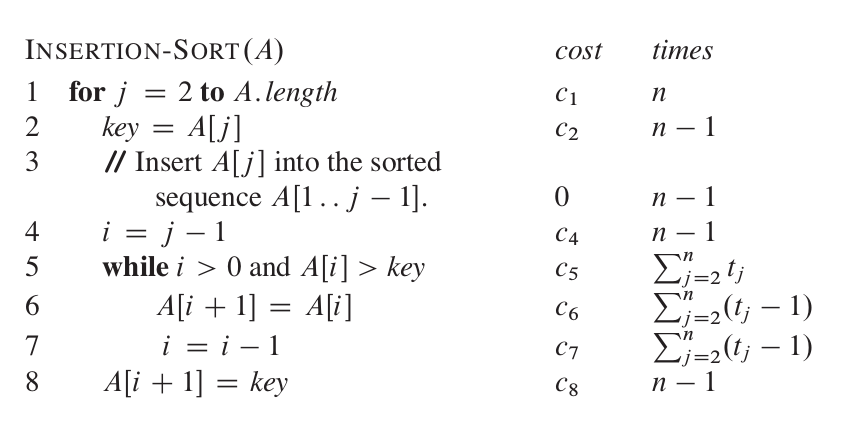
\includegraphics[height=5cm, width = 9cm]{./pic/insertionSort.png}
			\caption{Análise do Insertion Sort}
			\label{fig_analise_insertion}
		\end{figure}
	\end{block}
\end{frame}

%\begin{frame}	
%	\begin{block}{}	
%		 \begin{figure}[!htb]
%			\centering	  				
%			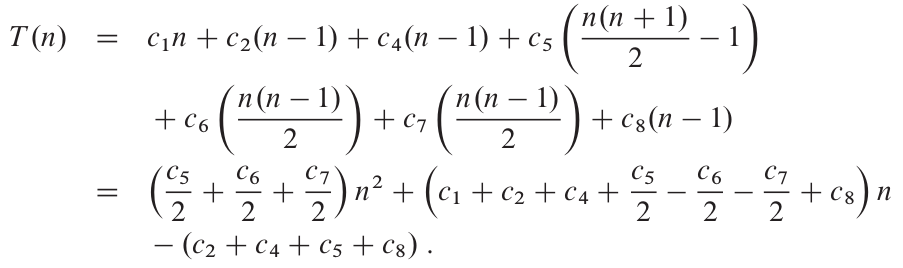
\includegraphics[height=4cm, width = 9cm]{./pic/custoInsertionSort.png}
%			\caption{Custo do Insertion Sort}
%			\label{fig_custo_insertion}
%		\end{figure}
%	\end{block}
%\end{frame}

\begin{frame}
\begin{block}{Uma aproximação do tempo de execução}
	\begin{itemize}
		\item Para valores grandes de entrada, quando n tende ao infinito, por exemplo. As constantes e termos de baixa ordem podem ser ignoradas.
		
		\item Uma proposta de aproximação é a notação assintótica que usa o termo de mais alta ordem para determinar o melhor, pior e caso médio de um algoritmo.
				
		\item Notação assintótica não depende da máquina onde o algoritmo vai executar apenas da contagem de passos internos do algoritmo.  Vamos analisar o InsertionSort com a notação assintótica.
		
	\end{itemize}
\end{block}
\end{frame}


\begin{frame}
\begin{block}{Notação assintótica}
	\begin{itemize}
		\item Não se assuste! É mais simples do que parece!

		\item Pior caso: $O(g(n))$ existem constantes positivas $c, n_0$ tal que $0 \leq f(n)  \leq cg(n)$ para todos $n \geq n_0$
				
		\item Melhor caso: $\Omega(g(n))$ existem constantes positivas $c, n_0$ tal que $0 \leq cg(n) \leq f(n)$ para todos $n \geq n_0$
				
		\item Caso médio: $\Theta(g(n))$ existem constantes positivas $c_1, c_2, n_0$ tal que $0 \leq c_1g(n) \leq f(n) \leq c_2g(n)$ para todos $n \geq n_0$
	\end{itemize}
\end{block}
\end{frame}

\begin{frame}	
	\begin{block}{Notação Assintótica}	
		 \begin{figure}[!htb]
			\centering	  				
			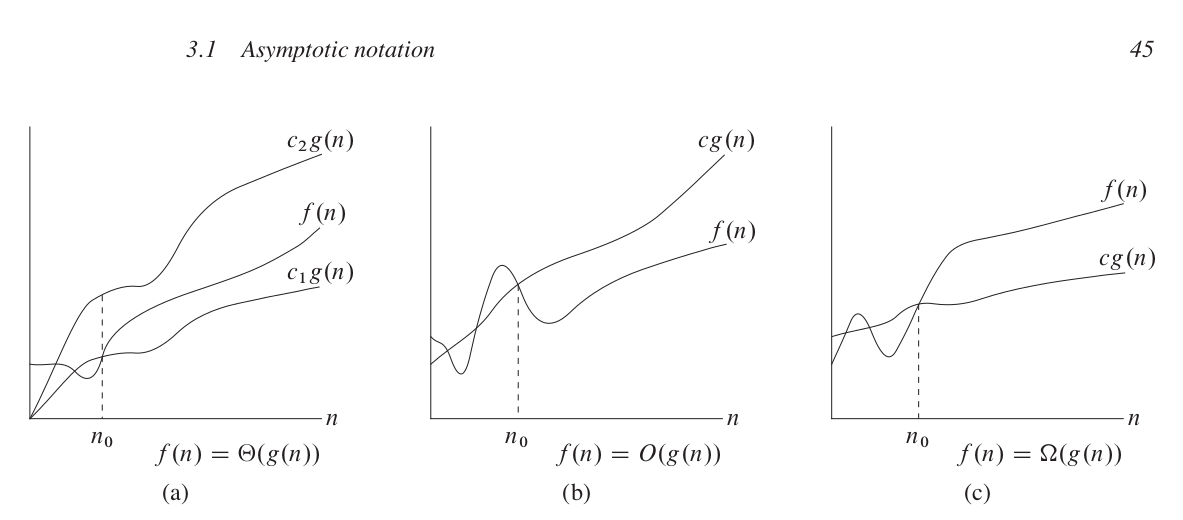
\includegraphics[height=4cm, width = 9cm]{./pic/analiseAssintotica.png}
			\caption{Notação Assintótica}
			\label{fig_analise_assintotica}
		\end{figure}
	\end{block}
\end{frame}


\begin{frame}[fragile]
	\begin{block}{Análise Busca Sequencial}	
				\inputminted[linenos,
									fontsize=\footnotesize,
									baselinestretch=1.2,
									framesep=2mm,
									bgcolor=bg_gray, 
									frame=lines]
									{csharp}
									{./secoes/AnaliseAlgoritmos/sequencialSearch.cs}
	\end{block}
\end{frame}

\begin{frame}
\begin{block}{Notação assintótica}
	\begin{itemize}
		\item Qual o melhor caso?
		\item Qual o pior caso?
		\item Qual o caso médio?
	\end{itemize}
\end{block}
\end{frame}

\begin{frame}[fragile]
	\begin{block}{Análise encontra mínimo}	
				\inputminted[linenos,
									fontsize=\footnotesize,
									baselinestretch=1.2,
									framesep=2mm,
									bgcolor=bg_gray, 
									frame=lines]
									{csharp}
									{./secoes/AnaliseAlgoritmos/encontraminimo.cs}
	\end{block}
\end{frame}